% Original pages: 33--40
% Figures: 1 unnumbered commutative diagram.
% Uncertainty log: none

\noindent\textit{Proposition 2.11.\amtarget{2.11} Let $0\longrightarrow M_0\longrightarrow M_1\longrightarrow\cdots\longrightarrow M_n\longrightarrow0$ be an exact sequence of $A$-modules in which all the modules $M_i$ and the kernels of all the homomorphisms belong to $C$. Then for any additive function $\lambda$ on $C$ we have}
\[
 \sum_{i=0}^n(-1)^i\lambda(M_i)=0.
\]

\noindent\textit{Proof.} Split up the sequence into short exact sequences
\[
 0\longrightarrow N_i\longrightarrow M_i\longrightarrow N_{i+1}\longrightarrow0
\]
($N_0=N_{n+1}=0$). Then we have $\lambda(M_i)=\lambda(N_i)+\lambda(N_{i+1})$. Now take the alternating sum of the $\lambda(M_i)$, and everything cancels out. \proofbox

\subsection{Tensor product of modules}

Let $M$, $N$, $P$ be three $A$-modules. A mapping $f:M\times N\longrightarrow P$ is said to be $A$-bilinear if for each $x\in M$ the mapping $y\mapsto f(x,y)$ of $N$ into $P$ is $A$-linear, and for each $y\in N$ the mapping $x\mapsto f(x,y)$ of $M$ into $P$ is $A$-linear.

We shall construct an $A$-module $T$, called the \textit{tensor product} of $M$ and $N$, with the property that the $A$-bilinear mappings $M\times N\longrightarrow P$ are in a natural one-to-one correspondence with the $A$-linear mappings $T\longrightarrow P$, for all $A$-modules $P$. More precisely:

\noindent\textit{Proposition 2.12.\amtarget{2.12} Let $M$, $N$ be $A$-modules. Then there exists a pair $(T,g)$ consisting of an $A$-module $T$ and an $A$-bilinear mapping $g:M\times N\longrightarrow T$, with the following property:}

\textit{Given any $A$-module $P$ and any $A$-bilinear mapping $f:M\times N\longrightarrow P$, there exists a unique $A$-linear mapping $f':T\longrightarrow P$ such that $f=f'\circ g$ (in other words, every bilinear function on $M\times N$ factors through $T$).}

\textit{Moreover, if $(T,g)$ and $(T',g')$ are two pairs with this property, then there exists a unique isomorphism $j:T\longrightarrow T'$ such that $j\circ g=g'$.}

\noindent\textit{Proof.} i) \textit{Uniqueness.} Replacing $(P,f)$ by $(T',g')$ we get a unique $j:T\longrightarrow T'$ such that $g'=j\circ g$. Interchanging the roles of $T$ and $T'$, we get $j':T'\longrightarrow T$ such that $g=j'\circ g'$. Each of the compositions $j\circ j'$, $j'\circ j$ must be the identity, and therefore $j$ is an isomorphism.

ii) \textit{Existence.} Let $C$ denote the free $A$-module $A^{(M\times N)}$. The elements of $C$ are formal linear combinations of elements of $M\times N$ with coefficients in $A$, i.e. they are expressions of the form $\sum_{i=1}^n a_i\cdot(x_i,y_i)$ ($a_i\in A$, $x_i\in M$, $y_i\in N$).

Let $D$ be the submodule of $C$ generated by all elements of $C$ of the following types:
\[
\begin{split}
(x+x',y)&-(x,y)-(x',y)\\
(x,y+y')&-(x,y)-(x,y')\\
(ax,y)&-a\cdot(x,y)\\
(x,ay)&-a\cdot(x,y).
\end{split}
\]

Let $T=C/D$. For each basis element $(x,y)$ of $C$, let $x\otimes y$ denote its image in $T$. Then $T$ is generated by the elements of the form $x\otimes y$, and from our definitions we have
\[
 (x+x')\otimes y=x\otimes y+x'\otimes y,\quad x\otimes(y+y')=x\otimes y+x\otimes y',
\]
\[
 (ax)\otimes y=x\otimes(ay)=a(x\otimes y).
\]
Equivalently, the mapping $g:M\times N\longrightarrow T$ defined by $g(x,y)=x\otimes y$ is $A$-bilinear.

Any map $f$ of $M\times N$ into an $A$-module $P$ extends by linearity to an $A$-module homomorphism $\bar f:C\longrightarrow P$. Suppose in particular that $f$ is $A$-bilinear. Then, from the definitions, $\bar f$ vanishes on all the generators of $D$, hence on the whole of $D$, and therefore induces a well-defined $A$-homomorphism $f'$ of $T=C/D$ into $P$ such that $f'(x\otimes y)=f(x,y)$. The mapping $f'$ is uniquely defined by this condition, and therefore the pair $(T,g)$ satisfy the conditions of the proposition. \proofbox

\noindent\textit{Remarks.} i) The module $T$ constructed above is called the \textit{tensor product} of $M$ and $N$, and is denoted by $M\otimes_A N$, or just $M\otimes N$ if there is no ambiguity about the ring $A$. It is generated as an $A$-module by the ``products'' $x\otimes y$. If $(x_i)_{i\in I}$, $(y_j)_{j\in J}$ are families of generators of $M$, $N$ respectively, then the elements $x_i\otimes y_j$ generate $M\otimes N$. In particular, if $M$ and $N$ are finitely generated, so is $M\otimes N$.

ii) The notation $x\otimes y$ is inherently ambiguous unless we specify the tensor product to which it belongs. Let $M'$, $N'$ be submodules of $M$, $N$ respectively, and let $x\in M'$ and $y\in N'$. Then it can happen that $x\otimes y$ as an element of $M\otimes N$ is zero whilst $x\otimes y$ as an element of $M'\otimes N'$ is non-zero. For example, take $A=\mathbb Z$, $M=\mathbb Z$, $N=\mathbb Z/2\mathbb Z$, and let $M'$ be the submodule $2\mathbb Z$ of $\mathbb Z$, whilst $N'=N$. Let $x$ be the non-zero element of $N$ and consider $2\otimes x$. As an element of $M\otimes N$, it is zero because $2\otimes x=1\otimes2x=1\otimes0=0$. But as an element of $M'\otimes N'$ it is non-zero. See the example after \amref{2.18}.

However, there is the following result:

\noindent\textit{Corollary 2.13.\amtarget{2.13} Let $x_i\in M$, $y_i\in N$ be such that $\sum x_i\otimes y_i=0$ in $M\otimes N$. Then there exist finitely generated submodules $M_0$ of $M$ and $N_0$ of $N$ such that $\sum x_i\otimes y_i=0$ in $M_0\otimes N_0$.}

\noindent\textit{Proof.} If $\sum x_i\otimes y_i=0$ in $M\otimes N$, then in the notation of the proof of \amref{2.12} we have $\sum(x_i,y_i)\in D$, and therefore $\sum(x_i,y_i)$ is a finite sum of generators of $D$. Let $M_0$ be the submodule of $M$ generated by the $x_i$ and all the elements of $M$ which occur as first coordinates in these generators of $D$, and define $N_0$ similarly. Then $\sum x_i\otimes y_i=0$ as an element of $M_0\otimes N_0$. \proofbox

iii) We shall never again need to use the construction of the tensor product given in \amref{2.12}, and the reader may safely forget it if he prefers. What is essential to keep in mind is the defining property of the tensor product.

iv) Instead of starting with bilinear mappings we could have started with multilinear mappings $f:M_1\times\cdots\times M_r\longrightarrow P$ defined in the same way (i.e., linear in each variable). Following through the proof of \amref{2.12} we should end up with a ``multi-tensor product'' $T=M_1\otimes\cdots\otimes M_r$, generated by all products $x_1\otimes\cdots\otimes x_r$ ($x_i\in M_i$, $1\leq i\leq r$). The details may safely be left to the reader; the result corresponding to \amref{2.12} is

\noindent\textit{Proposition 2.12*.\amtarget{2.12*} Let $M_1,\ldots,M_r$ be $A$-modules. Then there exists a pair $(T,g)$ consisting of an $A$-module $T$ and an $A$-multilinear mapping $g:M_1\times\cdots\times M_r\longrightarrow T$ with the following property:}

\textit{Given any $A$-module $P$ and any $A$-multilinear mapping $f:M_1\times\cdots\times M_r\longrightarrow T$, there exists a unique $A$-homomorphism $f':T\longrightarrow P$ such that $f'\circ g=f$.}

\textit{Moreover, if $(T,g)$ and $(T',g')$ are two pairs with this property, then there exists a unique isomorphism $j:T\longrightarrow T'$ such that $j\circ g=g'$.} \proofbox

There are various so-called ``canonical isomorphisms'', some of which we state here:

\noindent\textit{Proposition 2.14.\amtarget{2.14} Let $M$, $N$, $P$ be $A$-modules. Then there exist unique isomorphisms}
\begin{enumerate}
\renewcommand{\labelenumi}{\roman{enumi})}
\item $M\otimes N\longrightarrow N\otimes M$
\item $(M\otimes N)\otimes P\longrightarrow M\otimes(N\otimes P)\longrightarrow M\otimes N\otimes P$
\item $(M\oplus N)\otimes P\longrightarrow(M\otimes P)\oplus(N\otimes P)$
\item $A\otimes M\longrightarrow M$
\end{enumerate}
\textit{such that, respectively,}
\begin{enumerate}
\renewcommand{\labelenumi}{\alph{enumi})}
\item $x\otimes y\mapsto y\otimes x$
\item $(x\otimes y)\otimes z\mapsto x\otimes(y\otimes z)\mapsto x\otimes y\otimes z$
\item $(x,y)\otimes z\mapsto(x\otimes z,y\otimes z)$
\item $a\otimes x\mapsto ax$.
\end{enumerate}

\noindent\textit{Proof.} In each case the point is to show that the mappings so described are well defined. The technique is to construct suitable bilinear or multilinear mappings, and use the defining property \amref{2.12} or \amref{2.12*} to infer the existence of homomorphisms of tensor products. We shall prove half of ii) as an example of the method, and leave the rest to the reader.

We shall construct homomorphisms
\[
 (M\otimes N)\otimes P\xrightarrow{f}M\otimes N\otimes P\xrightarrow{g}(M\otimes N)\otimes P
\]
such that $f((x\otimes y)\otimes z)=x\otimes y\otimes z$ and $g(x\otimes y\otimes z)=(x\otimes y)\otimes z$ for all $x\in M$, $y\in N$, $z\in P$.

To construct $f$, fix the element $z\in P$. The mapping $(x,y)\mapsto x\otimes y\otimes z$ ($x\in M$, $y\in N$) is bilinear in $x$ and $y$ and therefore induces a homomorphism $f_z:M\otimes N\longrightarrow M\otimes N\otimes P$ such that $f_z(x\otimes y)=x\otimes y\otimes z$. Next, consider the mapping $(t,z)\mapsto f_z(t)$ of $(M\otimes N)\times P$ into $M\otimes N\otimes P$. This is bilinear in $t$ and $z$ and therefore induces a homomorphism
\[
 f:(M\otimes N)\otimes P\longrightarrow M\otimes N\otimes P
\]
such that $f((x\otimes y)\otimes z)=x\otimes y\otimes z$.

To construct $g$, consider the mapping $(x,y,z)\mapsto(x\otimes y)\otimes z$ of $M\times N\times P$ into $(M\otimes N)\otimes P$. This is linear in each variable and therefore induces a homomorphism
\[
 g:M\otimes N\otimes P\longrightarrow(M\otimes N)\otimes P
\]
such that $g(x\otimes y\otimes z)=(x\otimes y)\otimes z$.

Clearly $f\circ g$ and $g\circ f$ are identity maps, hence $f$ and $g$ are isomorphisms. \proofbox

\noindent\textit{Exercise 2.15.\amtarget{2.15} Let $A$, $B$ be rings, let $M$ be an $A$-module, $P$ a $B$-module and $N$ an $(A,B)$-bimodule (that is, $N$ is simultaneously an $A$-module and a $B$-module and the two structures are compatible in the sense that $a(xb)=(ax)b$ for all $a\in A$, $b\in B$, $x\in N$). Then $M\otimes_A N$ is naturally a $B$-module, $N\otimes_B P$ an $A$-module, and we have}
\[
 (M\otimes_A N)\otimes_B P\cong M\otimes_A(N\otimes_B P).
\]

Let $f:M\longrightarrow M'$, $g:N\longrightarrow N'$ be homomorphisms of $A$-modules. Define $h:M\times N\longrightarrow M'\otimes N'$ by $h(x,y)=f(x)\otimes g(y)$. It is easily checked that $h$ is $A$-bilinear and therefore induces an $A$-module homomorphism
\[
 f\otimes g:M\otimes N\longrightarrow M'\otimes N'
\]
such that
\[
 (f\otimes g)(x\otimes y)=f(x)\otimes g(y)\qquad(x\in M,\quad y\in N).
\]

Let $f':M'\longrightarrow M''$ and $g':N'\longrightarrow N''$ be homomorphisms of $A$-modules. Then clearly the homomorphisms $(f'\circ f)\otimes(g'\circ g)$ and $(f'\otimes g')\circ(f\otimes g)$ agree on all elements of the form $x\otimes y$ in $M\otimes N$. Since these elements generate $M\otimes N$, it follows that
\[
 (f'\circ f)\otimes(g'\circ g)=(f'\otimes g')\circ(f\otimes g).
\]

\subsection{Restriction and extension of scalars}

Let $f:A\longrightarrow B$ be a homomorphism of rings and let $N$ be a $B$-module. Then $N$ has an $A$-module structure defined as follows: if $a\in A$ and $x\in N$, then $ax$ is defined to be $f(a)x$. This $A$-module is said to be obtained from $N$ by \textit{restriction of scalars}. In particular, $f$ defines in this way an $A$-module structure on $B$.

\noindent\textit{Proposition 2.16.\amtarget{2.16} Suppose $N$ is finitely generated as a $B$-module and that $B$ is finitely generated as an $A$-module. Then $N$ is finitely generated as an $A$-module.}

\noindent\textit{Proof.} Let $y_1,\ldots,y_n$ generate $N$ over $B$, and let $x_1,\ldots,x_m$ generate $B$ as an $A$-module. Then the $mn$ products $x_i y_j$ generate $N$ over $A$. \proofbox

Now let $M$ be an $A$-module. Since, as we have just seen, $B$ can be regarded as an $A$-module, we can form the $A$-module $M_B=B\otimes_A M$. In fact $M_B$ carries a $B$-module structure such that $b(b'\otimes x)=bb'\otimes x$ for all $b,b'\in B$ and all $x\in M$. The $B$-module $M_B$ is said to be obtained from $M$ by \textit{extension of scalars}.

\noindent\textit{Proposition 2.17.\amtarget{2.17} If $M$ is finitely generated as an $A$-module, then $M_B$ is finitely generated as a $B$-module.}

\noindent\textit{Proof.} If $x_1,\ldots,x_m$ generate $M$ over $A$, then the $1\otimes x_i$ generate $M_B$ over $B$. \proofbox

\subsection{Exactness properties of the tensor product}

Let $f:M\times N\longrightarrow P$ be an $A$-bilinear mapping. For each $x\in M$ the mapping $y\mapsto f(x,y)$ of $N$ into $P$ is $A$-linear, hence $f$ gives rise to a mapping $M\longrightarrow\operatorname{Hom}(N,P)$ which is $A$-linear because $f$ is linear in the variable $x$. Conversely any $A$-homomorphism $\phi:M\longrightarrow\operatorname{Hom}_A(N,P)$ defines a bilinear map, namely $(x,y)\mapsto\phi(x)(y)$. Hence the set $S$ of $A$-bilinear mappings $M\times N\longrightarrow P$ is in natural one-to-one correspondence with $\operatorname{Hom}(M,\operatorname{Hom}(N,P))$. On the other hand $S$ is in one-to-one correspondence with $\operatorname{Hom}(M\otimes N,P)$, by the defining property of the tensor product. Hence we have a canonical isomorphism
\begin{equation}
 \operatorname{Hom}(M\otimes N,P)\cong\operatorname{Hom}(M,\operatorname{Hom}(N,P)).
 \tag{1}
\end{equation}

\noindent\textit{Proposition 2.18.\amtarget{2.18} Let}
\begin{equation}
 M'\xrightarrow{f}M\xrightarrow{g}M''\longrightarrow0
 \tag{2}
\end{equation}
\textit{be an exact sequence of $A$-modules and homomorphisms, and let $N$ be any $A$-module. Then the sequence}
\begin{equation}
 M'\otimes N\xrightarrow{f\otimes1}M\otimes N\xrightarrow{g\otimes1}M''\otimes N\longrightarrow0
 \tag{3}
\end{equation}
\textit{(where $1$ denotes the identity mapping on $N$) is exact.}

\noindent\textit{Proof.} Let $E$ denote the sequence (2), and let $E\otimes N$ denote the sequence (3). Let $P$ be any $A$-module. Since (2) is exact, the sequence $\operatorname{Hom}(E,\operatorname{Hom}(N,P))$ is exact by \amref{2.9}; hence by (1) the sequence $\operatorname{Hom}(E\otimes N,P)$ is exact. By \amref{2.9} again, it follows that $E\otimes N$ is exact. \proofbox

\noindent\textit{Remarks.} i) Let $T(M)=M\otimes N$ and let $U(P)=\operatorname{Hom}(N,P)$. Then (1) takes the form $\operatorname{Hom}(T(M),P)=\operatorname{Hom}(M,U(P))$ for all $A$-modules $M$ and $P$. In the language of abstract nonsense, the functor $T$ is the left adjoint of $U$, and $U$ is the right adjoint of $T$. The proof of \amref{2.18} shows that any functor which is a left adjoint is right exact. Likewise any functor which is a right adjoint is left exact.

ii) It is \textit{not} in general true that, if $M'\longrightarrow M\longrightarrow M''$ is an exact sequence of $A$-modules and homomorphisms, the sequence $M'\otimes N\longrightarrow M\otimes N\longrightarrow M''\otimes N$ obtained by tensoring with an arbitrary $A$-module $N$ is exact.

\noindent\textbf{Example.} Take $A=\mathbb Z$ and consider the exact sequence $0\longrightarrow\mathbb Z\xrightarrow{f}\mathbb Z$, where $f(x)=2x$ for all $x\in\mathbb Z$. If we tensor with $N=\mathbb Z/2\mathbb Z$, the sequence $0\longrightarrow\mathbb Z\otimes N\xrightarrow{f\otimes1}\mathbb Z\otimes N$ is not exact, because for any $x\otimes y\in\mathbb Z\otimes N$ we have
\[
 (f\otimes1)(x\otimes y)=2x\otimes y=x\otimes2y=x\otimes0=0,
\]
so that $f\otimes1$ is the zero mapping, whereas $\mathbb Z\otimes N\neq0$.

The functor $T_N:M\mapsto M\otimes_A N$ on the category of $A$-modules and homomorphisms is therefore not in general exact. If $T_N$ is exact, that is to say if tensoring with $N$ transforms all exact sequences into exact sequences, then $N$ is said to be a \textit{flat} $A$-module.

\noindent\textit{Proposition 2.19.\amtarget{2.19} The following are equivalent, for an $A$-module $N$:}
\begin{enumerate}
\renewcommand{\labelenumi}{\roman{enumi})}
\item \textit{$N$ is flat.}
\item \textit{If $0\longrightarrow M'\longrightarrow M\longrightarrow M''\longrightarrow0$ is any exact sequence of $A$-modules, the tensored sequence $0\longrightarrow M'\otimes N\longrightarrow M\otimes N\longrightarrow M''\otimes N\longrightarrow0$ is exact.}
\item \textit{If $f:M'\longrightarrow M$ is injective, then $f\otimes1:M'\otimes N\longrightarrow M\otimes N$ is injective.}
\item \textit{If $f:M'\longrightarrow M$ is injective and $M$, $M'$ are finitely generated, then $f\otimes1:M'\otimes N\longrightarrow M\otimes N$ is injective.}
\end{enumerate}

\noindent\textit{Proof.} i) $\Longleftrightarrow$ ii) by splitting up a long exact sequence into short exact sequences.

ii) $\Longleftrightarrow$ iii) by \amref{2.18}.

iii) $\Rightarrow$ iv): clear.

iv) $\Rightarrow$ iii). Let $f:M'\longrightarrow M$ be injective and let $u=\sum x_i'\otimes y_i\in\operatorname{Ker}(f\otimes1)$, so that $\sum f(x_i')\otimes y_i=0$ in $M\otimes N$. Let $M_0'$ be the submodule of $M'$ generated by the $x_i'$ and let $u_0$ denote $\sum x_i'\otimes y_i$ as an element of $M_0'\otimes N$. By \amref{2.14} there exists a finitely generated submodule $M_0$ of $M$ containing $f(M_0')$ and such that $\sum f(x_i')\otimes y_i=0$ as an element of $M_0\otimes N$. If $f_0:M_0'\longrightarrow M_0$ is the restriction of $f$, this means that $(f_0\otimes1)(u_0)=0$. Since $M_0$ and $M_0'$ are finitely generated, $f_0\otimes1$ is injective and therefore $u_0=0$, hence $u=0$. \proofbox

\noindent\textit{Exercise 2.20.\amtarget{2.20} If $f:A\longrightarrow B$ is a ring homomorphism and $M$ is a flat $A$-module, then $M_B=B\otimes_A M$ is a flat $B$-module.} (Use the canonical isomorphisms \amref{2.14}, \amref{2.15}.)

\subsection{Algebras}

Let $f:A\longrightarrow B$ be a ring homomorphism. If $a\in A$ and $b\in B$, define a product
\[
 ab=f(a)b.
\]
This definition of scalar multiplication makes the ring $B$ into an $A$-module (it is a particular example of restriction of scalars). Thus $B$ has an $A$-module structure as well as a ring structure, and these two structures are compatible in a sense which the reader will be able to formulate for himself. The ring $B$, equipped with this $A$-module structure, is said to be an $A$-algebra. Thus an $A$-algebra is, by definition, a ring $B$ together with a ring homomorphism $f:A\longrightarrow B$.

\noindent\textit{Remarks.} i) In particular, if $A$ is a field $K$ (and $B\neq0$) then $f$ is injective by \amref{1.2} and therefore $K$ can be canonically identified with its image in $B$. Thus a $K$-algebra ($K$ a field) is effectively a ring containing $K$ as a subring.

ii) Let $A$ be any ring. Since $A$ has an identity element there is a unique homomorphism of the ring of integers $\mathbb Z$ into $A$, namely $n\mapsto n\cdot1$. Thus every ring is automatically a $\mathbb Z$-algebra.

Let $f:A\longrightarrow B$, $g:A\longrightarrow C$ be two ring homomorphisms. An $A$-algebra homomorphism $h:B\longrightarrow C$ is a ring homomorphism which is also an $A$-module homomorphism. The reader should verify that $h$ is an $A$-algebra homomorphism if and only if $h\circ f=g$.

A ring homomorphism $f:A\longrightarrow B$ is \textit{finite}, and $B$ is a \textit{finite $A$-algebra}, if $B$ is finitely generated as an $A$-module. The homomorphism $f$ is \textit{of finite type}, and $B$ is a \textit{finitely-generated $A$-algebra}, if there exists a finite set of elements $x_1,\ldots,x_n$ in $B$ such that every element of $B$ can be written as a polynomial in $x_1,\ldots,x_n$ with coefficients in $f(A)$; or equivalently if there is an $A$-algebra homomorphism from a polynomial ring $A[t_1,\ldots,t_n]$ onto $B$.

A ring $A$ is said to be \textit{finitely generated} if it is finitely generated as a $\mathbb Z$-algebra. This means that there exist finitely many elements $x_1,\ldots,x_n$ in $A$ such that every element of $A$ can be written as a polynomial in the $x_i$ with rational integer coefficients.

\subsection{Tensor product of algebras}

Let $B$, $C$ be two $A$-algebras, $f:A\longrightarrow B$, $g:A\longrightarrow C$ the corresponding homomorphisms. Since $B$ and $C$ are $A$-modules we may form their tensor product $D=B\otimes_A C$, which is an $A$-module. We shall now define a multiplication on $D$.

Consider the mapping $B\times C\times B\times C\longrightarrow D$ defined by
\[
 (b,c,b',c')\mapsto bb'\otimes cc'.
\]
This is $A$-linear in each factor and therefore, by \amref{2.12*}, induces an $A$-module homomorphism
\[
 B\otimes C\otimes B\otimes C\longrightarrow D,
\]
hence by \amref{2.14} an $A$-module homomorphism
\[
 D\otimes D\longrightarrow D
\]
and this in turn by \amref{2.11} corresponds to an $A$-bilinear mapping
\[
 \mu:D\times D\longrightarrow D
\]
which is such that
\[
 \mu(b\otimes c,b'\otimes c')=bb'\otimes cc'.
\]
Of course, we could have written down this formula directly, but without some such argument as we have given there would be no guarantee that $\mu$ was well-defined.

We have therefore defined a multiplication on the tensor product $D=B\otimes_A C$: for elements of the form $b\otimes c$ it is given by
\[
 (b\otimes c)(b'\otimes c')=bb'\otimes cc',
\]
and in general by
\[
 \left(\sum_i(b_i\otimes c_i)\right)\left(\sum_j(b_j'\otimes c_j')\right)
 =\sum_{i,j}(b_i b_j'\otimes c_i c_j').
\]
The reader should check that with this multiplication $D$ is a commutative ring, with identity element $1\otimes1$. Furthermore, $D$ is an $A$-algebra: the mapping $a\mapsto f(a)\otimes g(a)$ is a ring homomorphism $A\longrightarrow D$.

In fact there is a commutative diagram of ring homomorphisms

\begin{center}
% Unnumbered commutative diagram from original page 40.
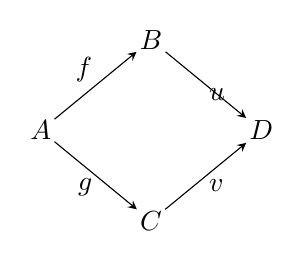
\begin{tikzpicture}[
  baseline=(current bounding box.center),
  every node/.style={inner sep=1pt},
  every path/.style={->,>=stealth}
]
  \node (A) at (0,0) {$A$};
  \node (B) at (1.4,1.15) {$B$};
  \node (C) at (1.4,-1.15) {$C$};
  \node (D) at (2.8,0) {$D$};

  \draw (A) -- node[above left] {$f$} (B);
  \draw (A) -- node[below left] {$g$} (C);
  \draw (B) -- node[below right] {$u$} (D);
  \draw (C) -- node[below right] {$v$} (D);
\end{tikzpicture}

\end{center}

in which $u$, for example, is defined by $u(b)=b\otimes1$.

\subsection{Exercises}

\begin{enumerate}
\item Show that $(\mathbb Z/m\mathbb Z)\otimes_{\mathbb Z}(\mathbb Z/n\mathbb Z)=0$ if $m$, $n$ are coprime.

\amstaritem Let $A$ be a ring, $\mathfrak a$ an ideal, $M$ an $A$-module. Show that $(A/\mathfrak a)\otimes_A M$ is isomorphic to $M/\mathfrak aM$.

[Tensor the exact sequence $0\longrightarrow\mathfrak a\longrightarrow A\longrightarrow A/\mathfrak a\longrightarrow0$ with $M$.]

\amstaritem Let $A$ be a local ring, $M$ and $N$ finitely generated $A$-modules. Prove that if $M\otimes N=0$, then $M=0$ or $N=0$.

[Let $\mathfrak m$ be the maximal ideal, $k=A/\mathfrak m$ the residue field. Let $M_k=k\otimes_A M\cong M/\mathfrak mM$ by Exercise 2. By Nakayama's lemma, $M_k=0\Rightarrow M=0$. But $M\otimes_A N=0\Rightarrow(M\otimes_A N)_k=0\Rightarrow M_k\otimes_k N_k=0\Rightarrow M_k=0$ or $N_k=0$, since $M_k$, $N_k$ are vector spaces over a field.]

\amstaritem Let $M_i$ ($i\in I$) be any family of $A$-modules, and let $M$ be their direct sum. Prove that $M$ is flat $\Longleftrightarrow$ each $M_i$ is flat.
\end{enumerate}
